\section{Charakterystyka próby badawczej} 
Ostatecznie zgromadzono pełne odpowiedzi od 74 respondentów. Ankietę rozpoczęło, a nie dokończyło 50 osób. Co oznacza, że $40.32\%$ osób odpadło na etapie wypełniania ankiety. 

Z 74 pełnych odpowiedzi zdecydowano się na odrzucenie 1 respondenta ze względu na nieprawidłowy charakter otrzymanych danych. Dla testu \emph{UWES} wszystkie odpowiedzi były 0 (nigdy), dla pierwszej połowy testu \emph{JSS} wszystkie odpowiedzi były 1 (,,zdecydowanie się nie zgadzam"), natomiast dla drugiej połowy -- 6 (,,zdecydowanie się zgadzam"). Z czego wynika, że na każdej wyświetlanej w przeglądarce stronie ankiety respondent odpowiadał tak samo. Jest bardzo mało
prawdopodobnym, aby taki charakter miały jego prawdziwe odczucia oraz stosunek do pracy. Ze względu na to dane zostały uznane za błędne i odrzucone.
\subsection{Płeć}
Większość respondentów to mężczyźni -- 62 osoby ($84.93\%$). Tylko 11 ($15.07\%$) osób to były kobiety. Stosunek ten nie jest zaskakujący ze względu na charakter pracy. Większość pracowników sektora IT to mężczyźni. Dla przykładu, w Dziale Usług Sieciowych Poznańskiego Centrum Superkomputerowo-Sieciowego, na prawie 100 pracowników technicznych, tylko 5 to kobiety.

\begin{figure}[h]
\begin{center}
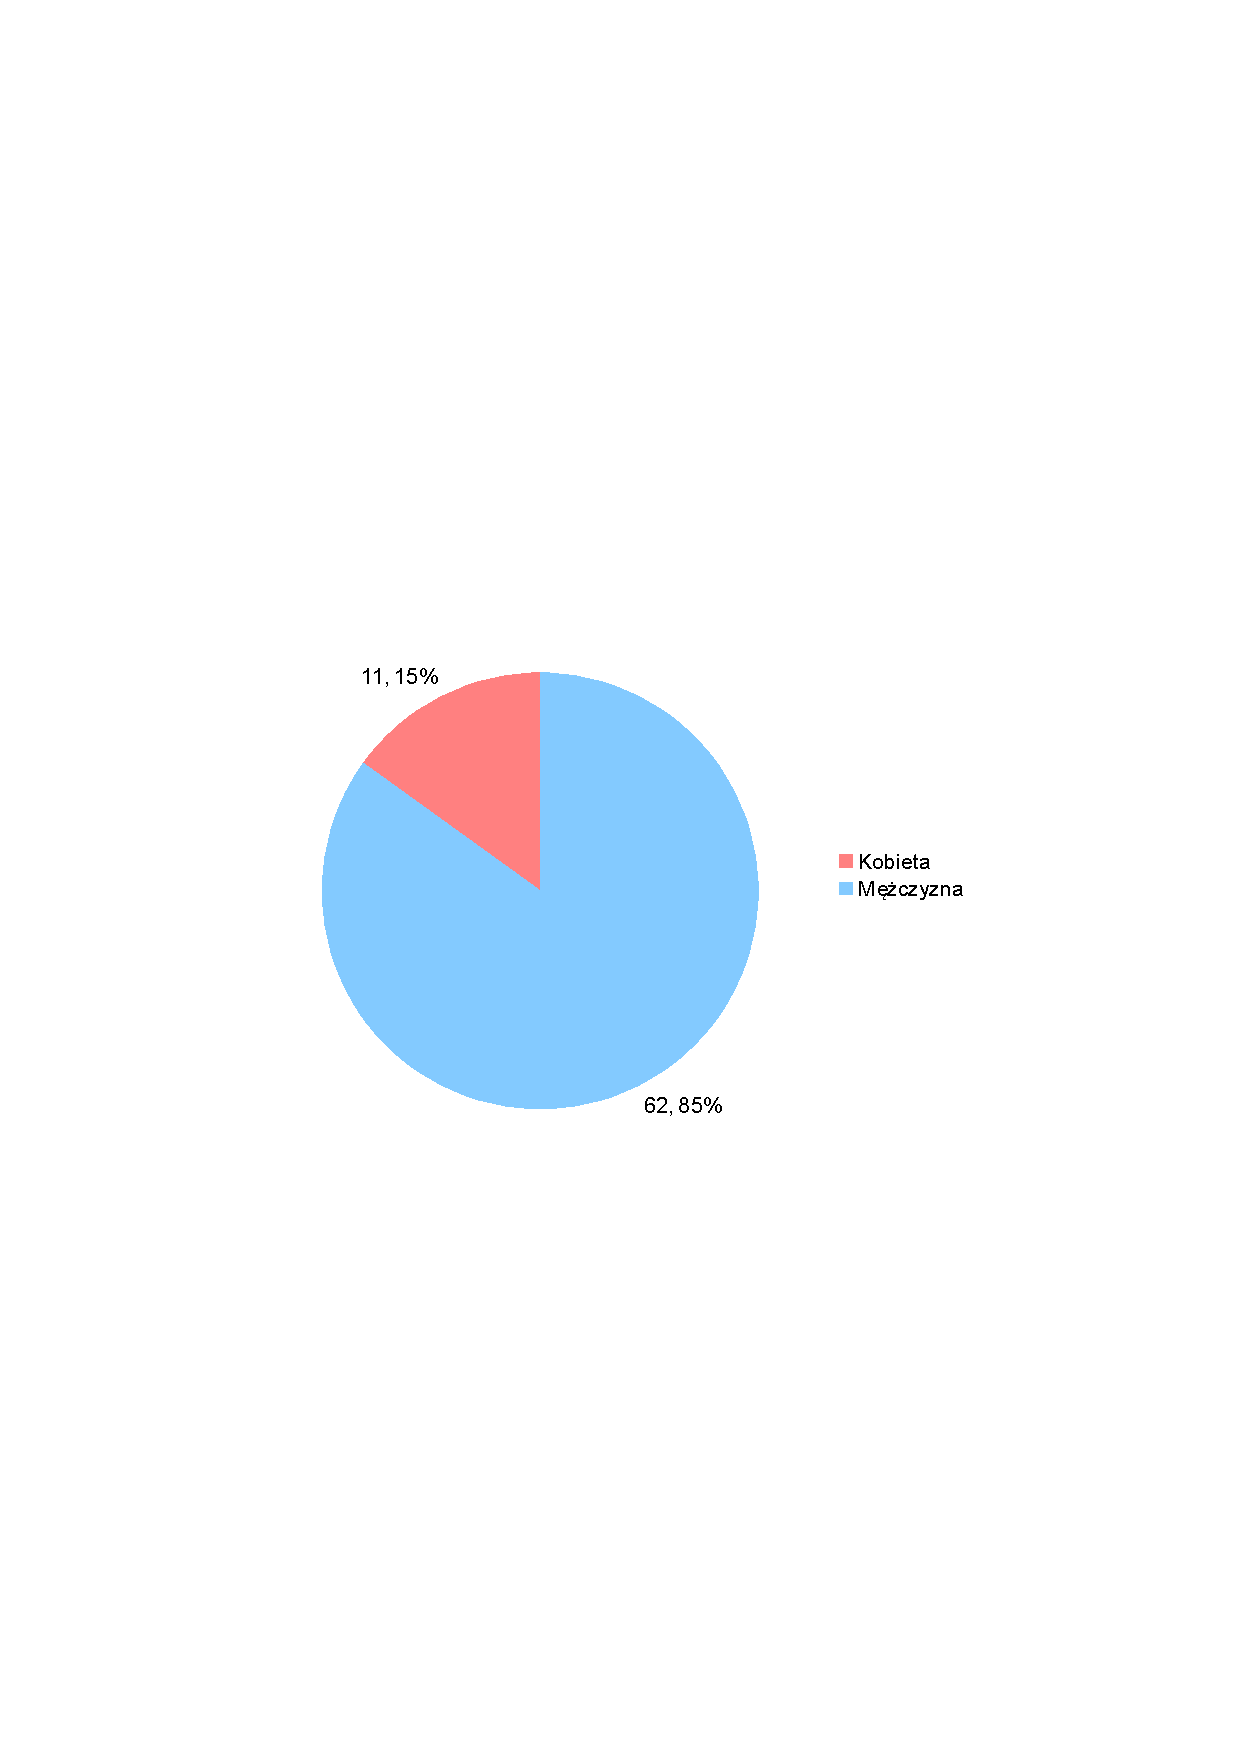
\includegraphics[width=0.6\textwidth]{sex}
\end{center}
\caption{Płeć respondentów.}
\label{fig:sex}
\end{figure}

\subsection{Wiek}
Badanie zgromadziło osoby w wieku od 22 do 37 lat. Na podstawie danych z Tabeli \ref{tab:age-stats} możemy zawuażyć, że ok. trzy-czwarte osób to osoby poniżej 30 roku życia (wiek 30 to trzeci kwartyl). Po dokładniejszym sprawdzeniu okazuje się, że w wieku 30 i mniej lat jest prawie $80\%$ osób.  Najczęściej występujący wiek to 26, natomiast wiek rozdzielający grupę badanych na pół to 27. Liczby te dają obraz jak młoda jest grupa badanych. 

\begin{table}[h!]
\begin{center}
\begin{tabular}{c c c c c c c}
Min. & 1 kwartyl & Mediana & 3 kwartyl & Max. & Śr. & Moda \\ \hline
22 & 26 & 27 & 30 & 37 & 28,37 & 26 \\
\end{tabular}
\end{center}
\caption{Statystyki odnośnie wieku respondentów.}
\label{tab:age-stats}
\end{table}

Dodatkowo jeżeli zawęzimy przedział do osób między 25, a 28 rokiem życia (czteroletni przedział), to w wyniku otrzymujemy 46 osób, które stanowią ponad dwie-trzecie grupy badanych (patrz Rysunek \ref{fig:age}).

\begin{figure}[h]
\begin{center}
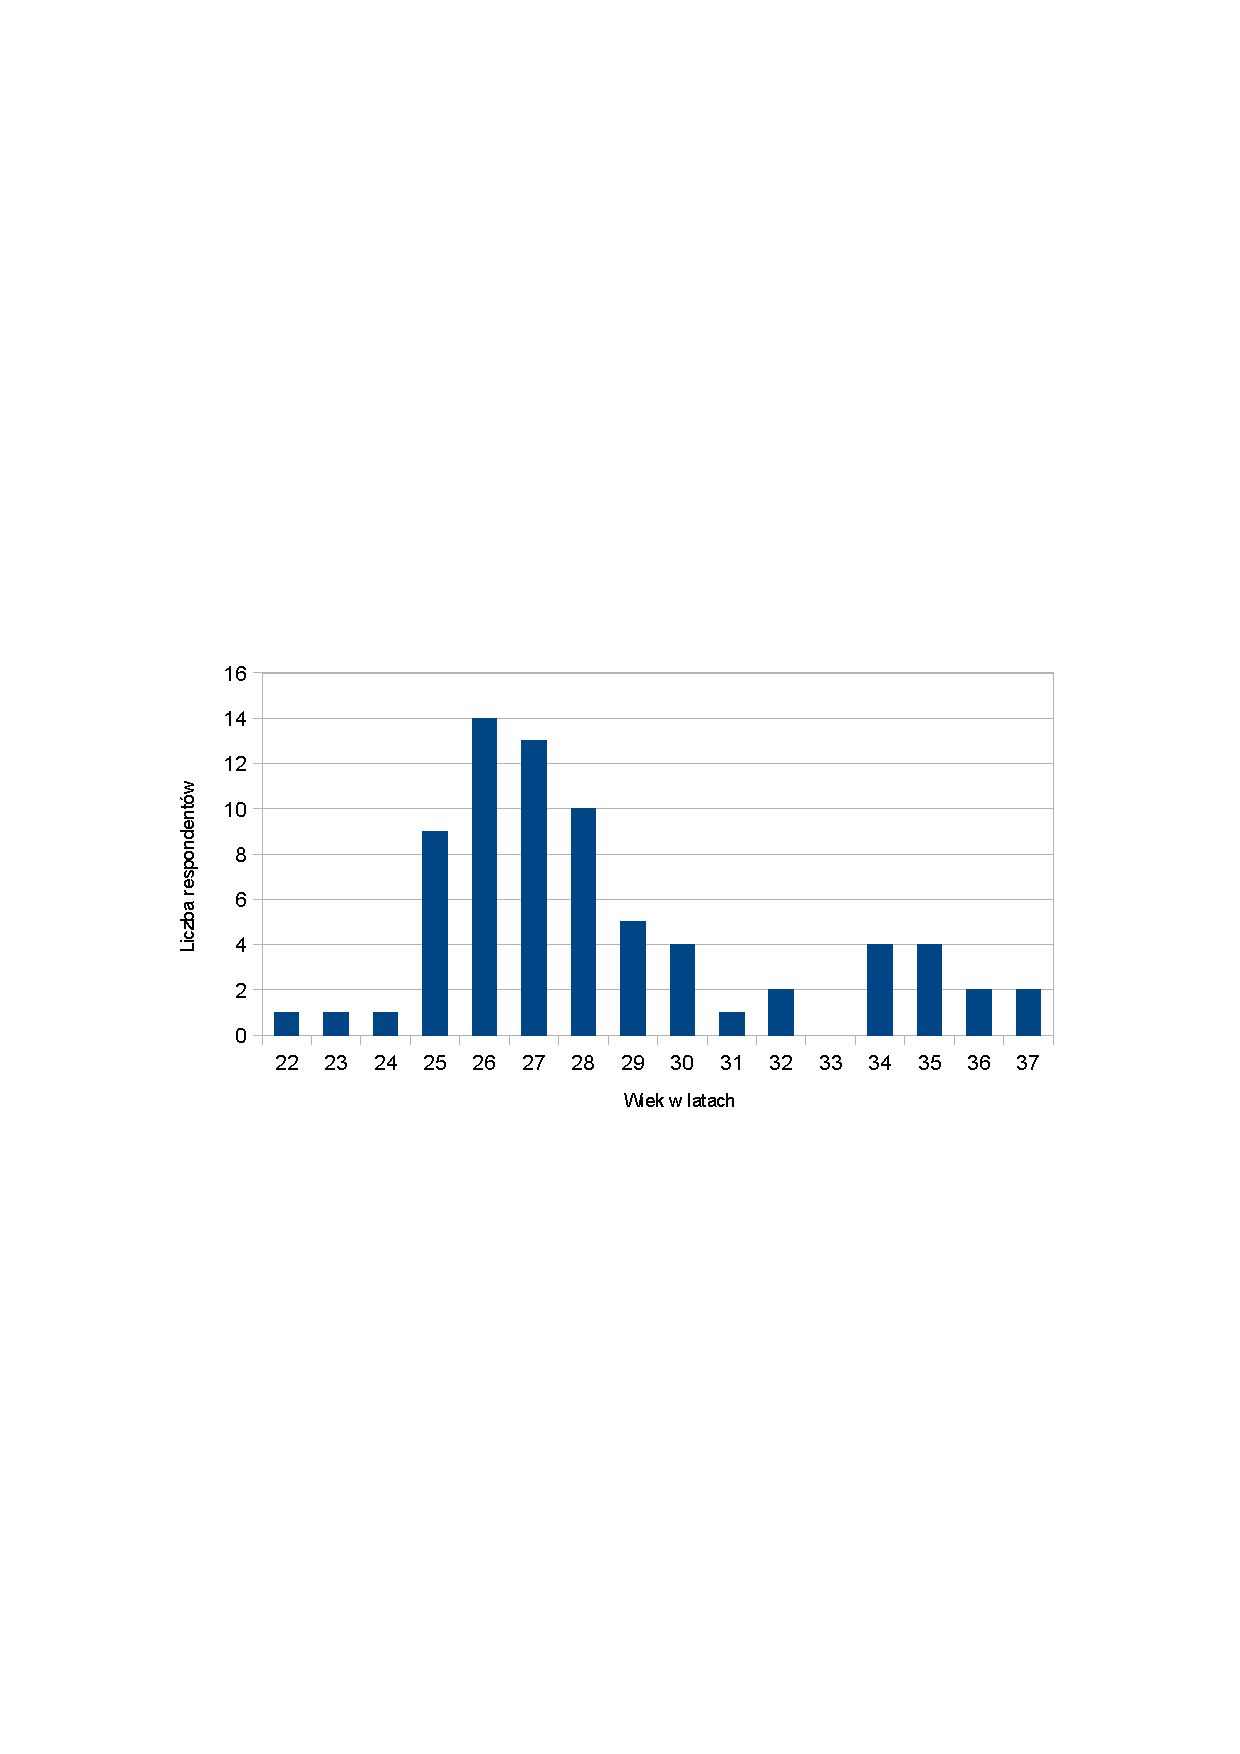
\includegraphics[width=0.8\textwidth]{age}
\end{center}
\caption{Histogram wieku respondentów.}
\label{fig:age}
\end{figure}

\subsection{Doświadczenie}

\begin{table}[h!]
\begin{center}
\begin{tabular}{c c c c c c c}
Min. & 1 kwartyl & Mediana & 3 kwartyl & Max. & Śr. & Moda \\ \hline
0 & 1 & 2 & 4 & 13 & 3,11 & 1 \\
\end{tabular}
\end{center}
\caption{Statystyki odnośnie doświadczenia respondentów.}
\label{tab:expierience-stats}
\end{table}

Jak widać z danych statystycznych, najwięcej osób posiada doświadczenie 1 roku (28 osób). Co najmniej połowa respondentów pracuje co najwyżej 2 lata, a trzy czwarte -- 4 lata. Średnia to trochę ponad 3 lata, ale jest ona zaburzona poprzez wartości odstające (patrza Rysunek \ref{fig:expierience}). Osoby z doświadczeniem od 8 do 13 lat to tylko 12,33\% (9 osób) grupy.

\begin{figure}[h]
\begin{center}
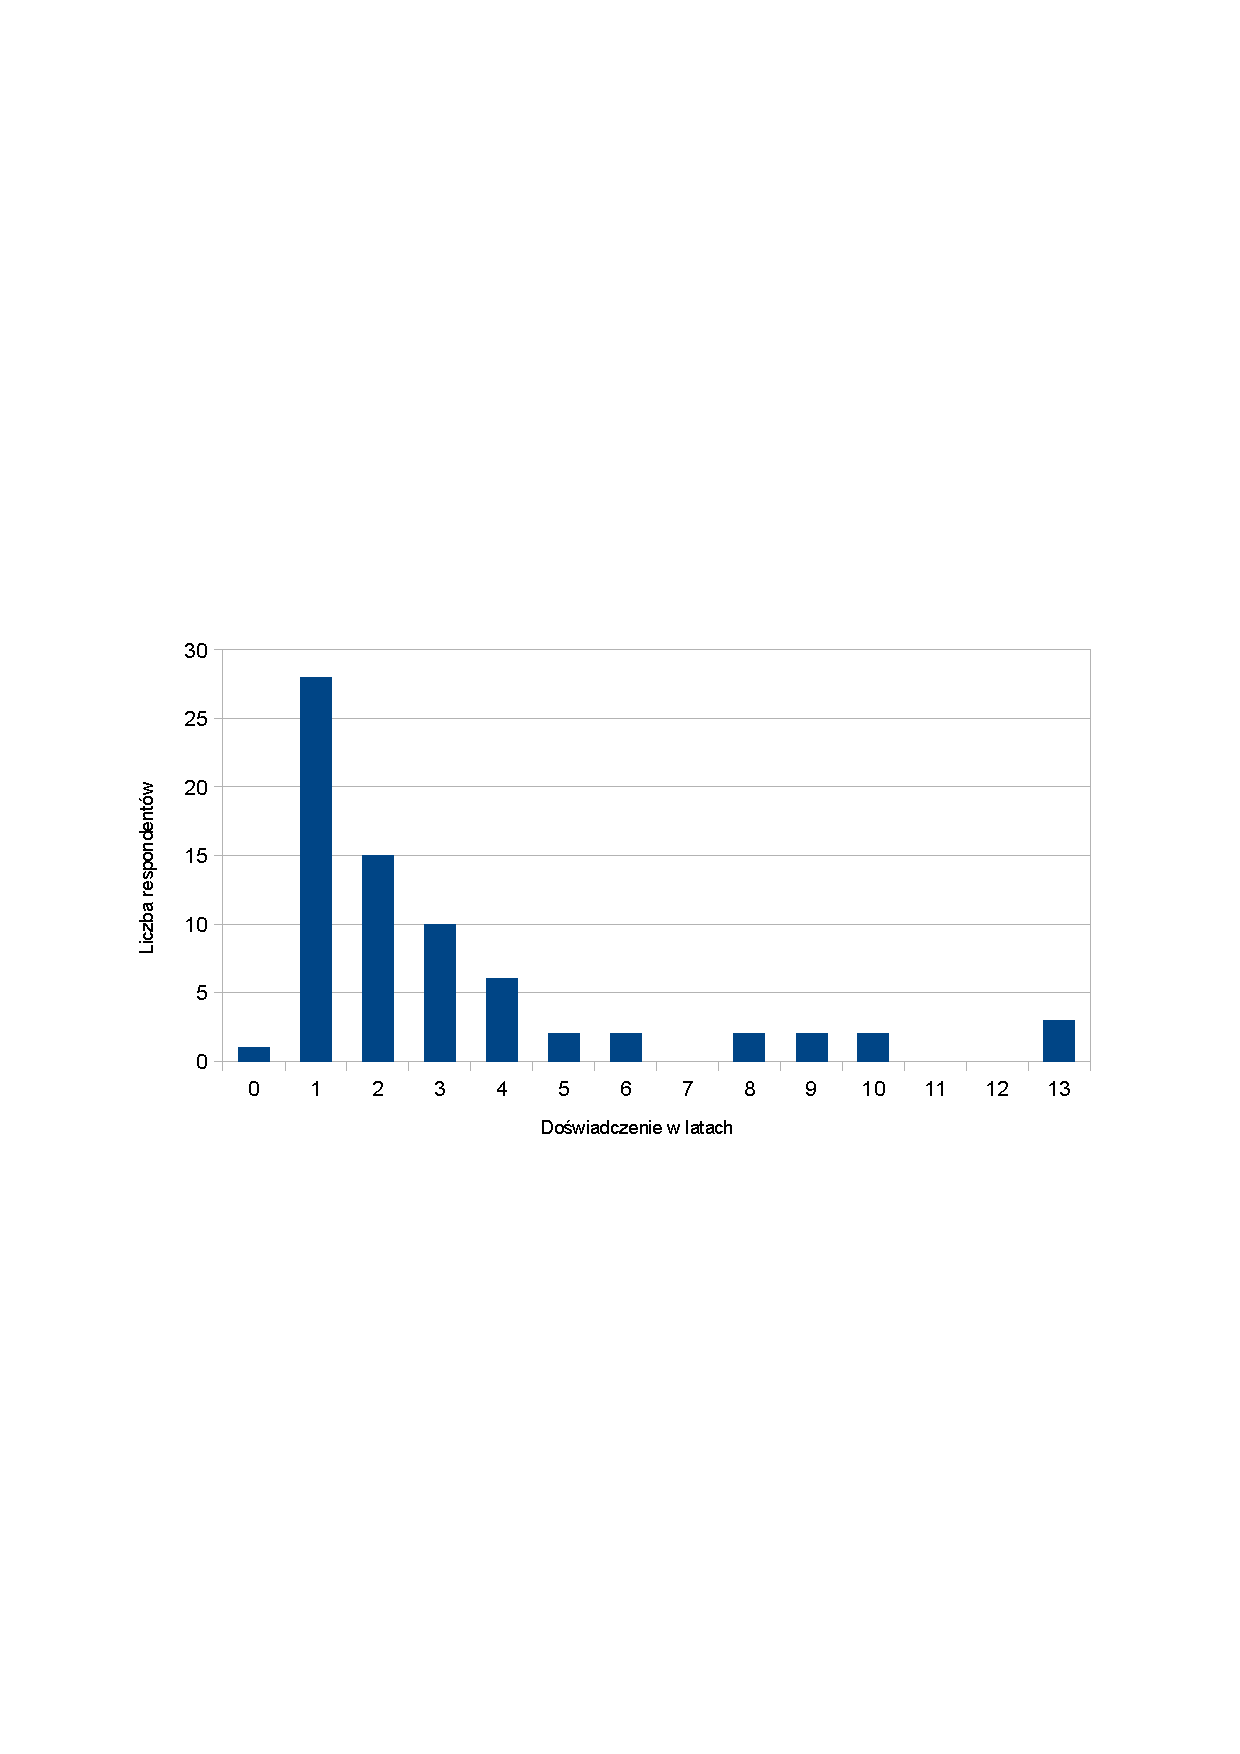
\includegraphics[width=0.8\textwidth]{expierience}
\end{center}
\caption{Histogram doświadczenia respondentów.}
\label{fig:expierience}
\end{figure}

Wynika z tego, że większość osób badanych posiada krótkie doświadczenie zawodowe. Podkreślają to statystyki odnośnie ilości osób mających doświadczenie między 1 rokiem, a 4 latami (59 osób; 80,82\%).

\subsection{Obecne stanowisko}

\begin{table}[h!]
\begin{center}
\begin{tabular}{l r r}
Stanowisko & Liczba & Procent \\ \hline
pracownik szeregowy & 6 & 8,22\% \\
młodszy specjalista & 8 & 10,96\% \\
specjalista & 34 & 46,58\% \\
starszy specjalista & 15 & 20,55\% \\
kierownik zespołu & 8 & 10,96\% \\
kierownik średniego szczebla & 1 & 1,37\% \\
wyższa kadra kierownicza & 1 & 1,37\% \\
\end{tabular}
\end{center}
\caption{Statystyki odnośnie obecnego stanowiska.}
\label{tab:position-stats}
\end{table}

Zdecydowana większość osób pracuje jako specjalista różnego szczebla (57 osób; 78,08\%). Przewagę tej grupy widać wyraźnie na Rysunku \ref{fig:position}. Są to osoby zajmujące się czysto technicznymi aspektami wykonywanej pracy, a co za tym idzie nie odpowiadają za zarządzanie ludźmi ani kontakty z klientem. Natomiast kierownicy stanowią 13,70\% (10 osób) grupy badanych. Tylko 6 osób (8,22\%) określiło siebie jako pracownik szeregowy.

\begin{figure}[h]
\begin{center}
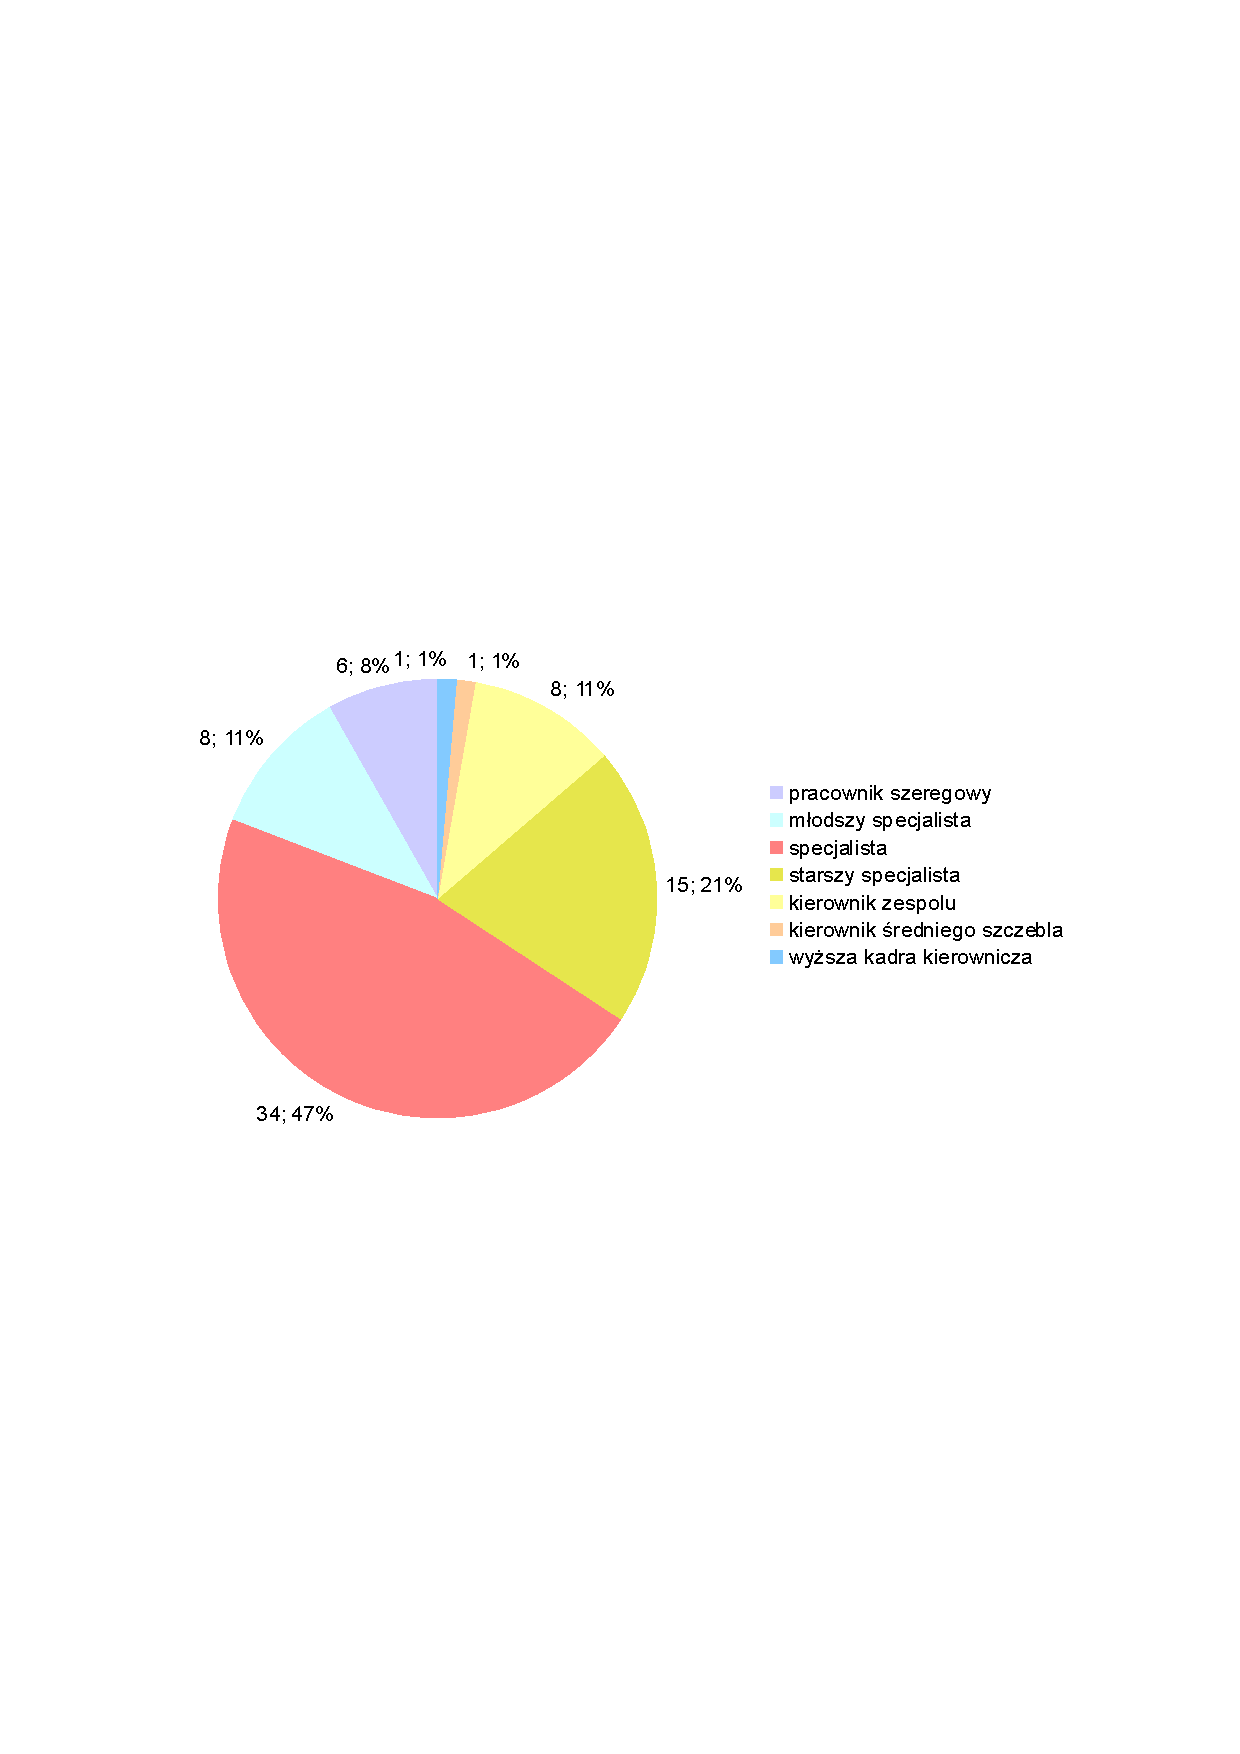
\includegraphics[width=0.8\textwidth]{position}
\end{center}
\caption{Wykres stanowisk respondentów.}
\label{fig:position}
\end{figure}

\begin{table}[h!]
\begin{center}
\begin{tabular}{c c c c c c c}
Min. & 1 kwartyl & Mediana & 3 kwartyl & Max. & Śr. & Moda \\ \hline
0 & 1 & 2 & 3 & 13 & 2,23 & 1 \\
\end{tabular}
\end{center}
\caption{Statystyki odnośnie stażu pracy na obecnym stanowisku.}
\label{tab:position-years-stats}
\end{table}

Patrząc na statystyki z Tabeli \ref{tab:position-years-stats} widzimy, że po ok. 25\% grupy stanowią osoby pracujące 1 rok, 2 lata lub 3 lata. Jeżeli przyjrzymy się bliżej histogramowi na Rysunku \ref{fig:position-years} możemy zauważyć, że najczęstsza wartość -- 1 rok, powtarza się aż 33 razy. Oznacza to, że grupa badanych dopiero nabiera doświadczenia na obecnych stanowiskach. Są one dla nich nowe i ekscytujące.

\begin{figure}[h]
\begin{center}
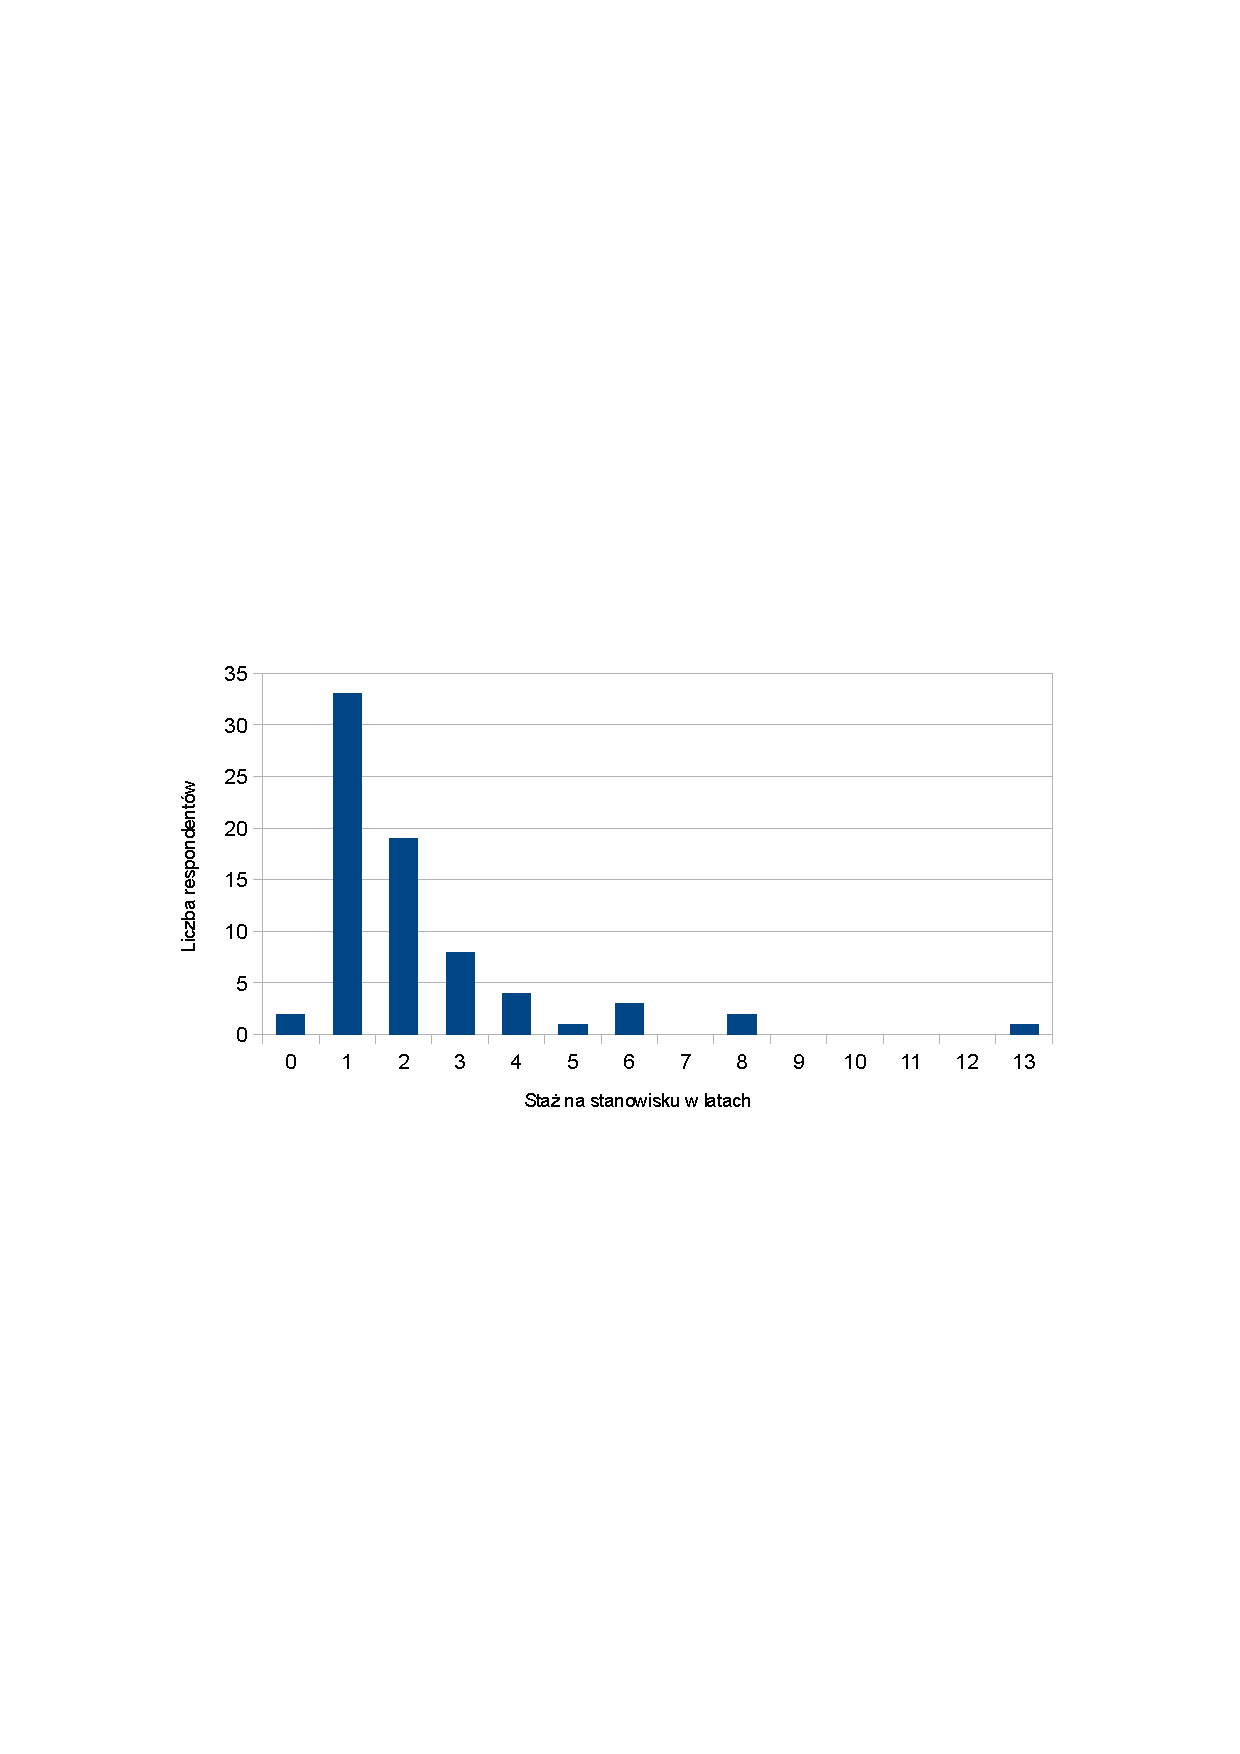
\includegraphics[width=0.8\textwidth]{position-years}
\end{center}
\caption{Histogram stażu pracy na obecnym stanowisku.}
\label{fig:position-years}
\end{figure}

Interesującą wartością jest wartość maksymalna -- 13 lat na obecnym stanowisku. Wartość ta pokrywa się z maksymalną wartością doświadczenia. Po dokładniejszym przyjrzeniu się danym, okazało się, że jest to 36-letni mężczyzna, który przez cały ten okres zajmuje pozycję pracownika szeregowego. Może się to wiązać faktycznie z brakiem awansów. Jednak bardziej prawdopodobne wydaje się praca dla firmy, w której brakuje jasnej struktury podziału
pozycji pracowników.

\subsection{Forma zatrudnienia}

\begin{table}[h!]
\begin{center}
\begin{tabular}{l r r}
Etat & Liczba & Procent \\ \hline
praca na cały etat & 68 & 93,15\% \\
praca na trzy-czwarte etatu & 0 & 0\% \\
praca na pół etatu & 2 & 2,74\% \\
inne & 3 & 4,11\% \\
\end{tabular}
\end{center}
\caption{Rodzaj etatu wśród respondentów.}
\label{tab:work-time-stats}
\end{table}

Jak widać w Tabeli \ref{tab:work-time-stats} prawie wszyscy respondenci (68 osób; 93,15\%) pracują na cały etat. Nie ma nikogo na trzy-czwarte etatu i tylko 2 osoby (2,74\%) na pół etatu. Co ciekawe 3 osoby (4,11\%) wskazało na inną formę etatu. Prawdopodobnie osoby te mają nieregulowany czas pracy. Wskazuje to na osoby samozatrudniające się lub na firmy, gdzie 40-godzinny tydzień pracy nie jest przestrzegany.

\begin{table}[h!]
\begin{center}
\begin{tabular}{l r r}
Umowa & Liczba & Procent \\ \hline
umowa o pracę & 57 & 78,08\% \\
umowa zlecenie & 3 & 4,11\% \\
umowa o dzieło & 0 & 0\% \\
samozatrudnienie & 8 & 10,96\% \\
umowa o pracę i dzieło & 5 & 6,85\% \\
\end{tabular}
\end{center}
\caption{Rodzaj zastrudnienia wśród respondentów.}
\label{tab:work-time-stats}
\end{table}

Analizując dane z Tabeli \ref{tab:work-time-stats} można zauważyć, że ponad trzy-czwarte grupy (57 osób) pracuje na umowę o pracę. Stanowi ona obecnie najbezpieczniejszą formę zatrudnienia jeżeli chodzi o świadczenia i prawa pracowników. Na umowę zlecenie pracują tylko 3 osoby. Liczba ta pokrywa się z osobami pracującymi nie na etat (w polu ,,etat" wybrano ,,inne"). Po przyjrzeniu się źródłowym danym, żadna z tych osób nie wybrała tego pola. Natomiast 1 osoba z
samozatrudnionych wybrała ,,inny etat". 

\begin{figure}[htb]
\begin{center}
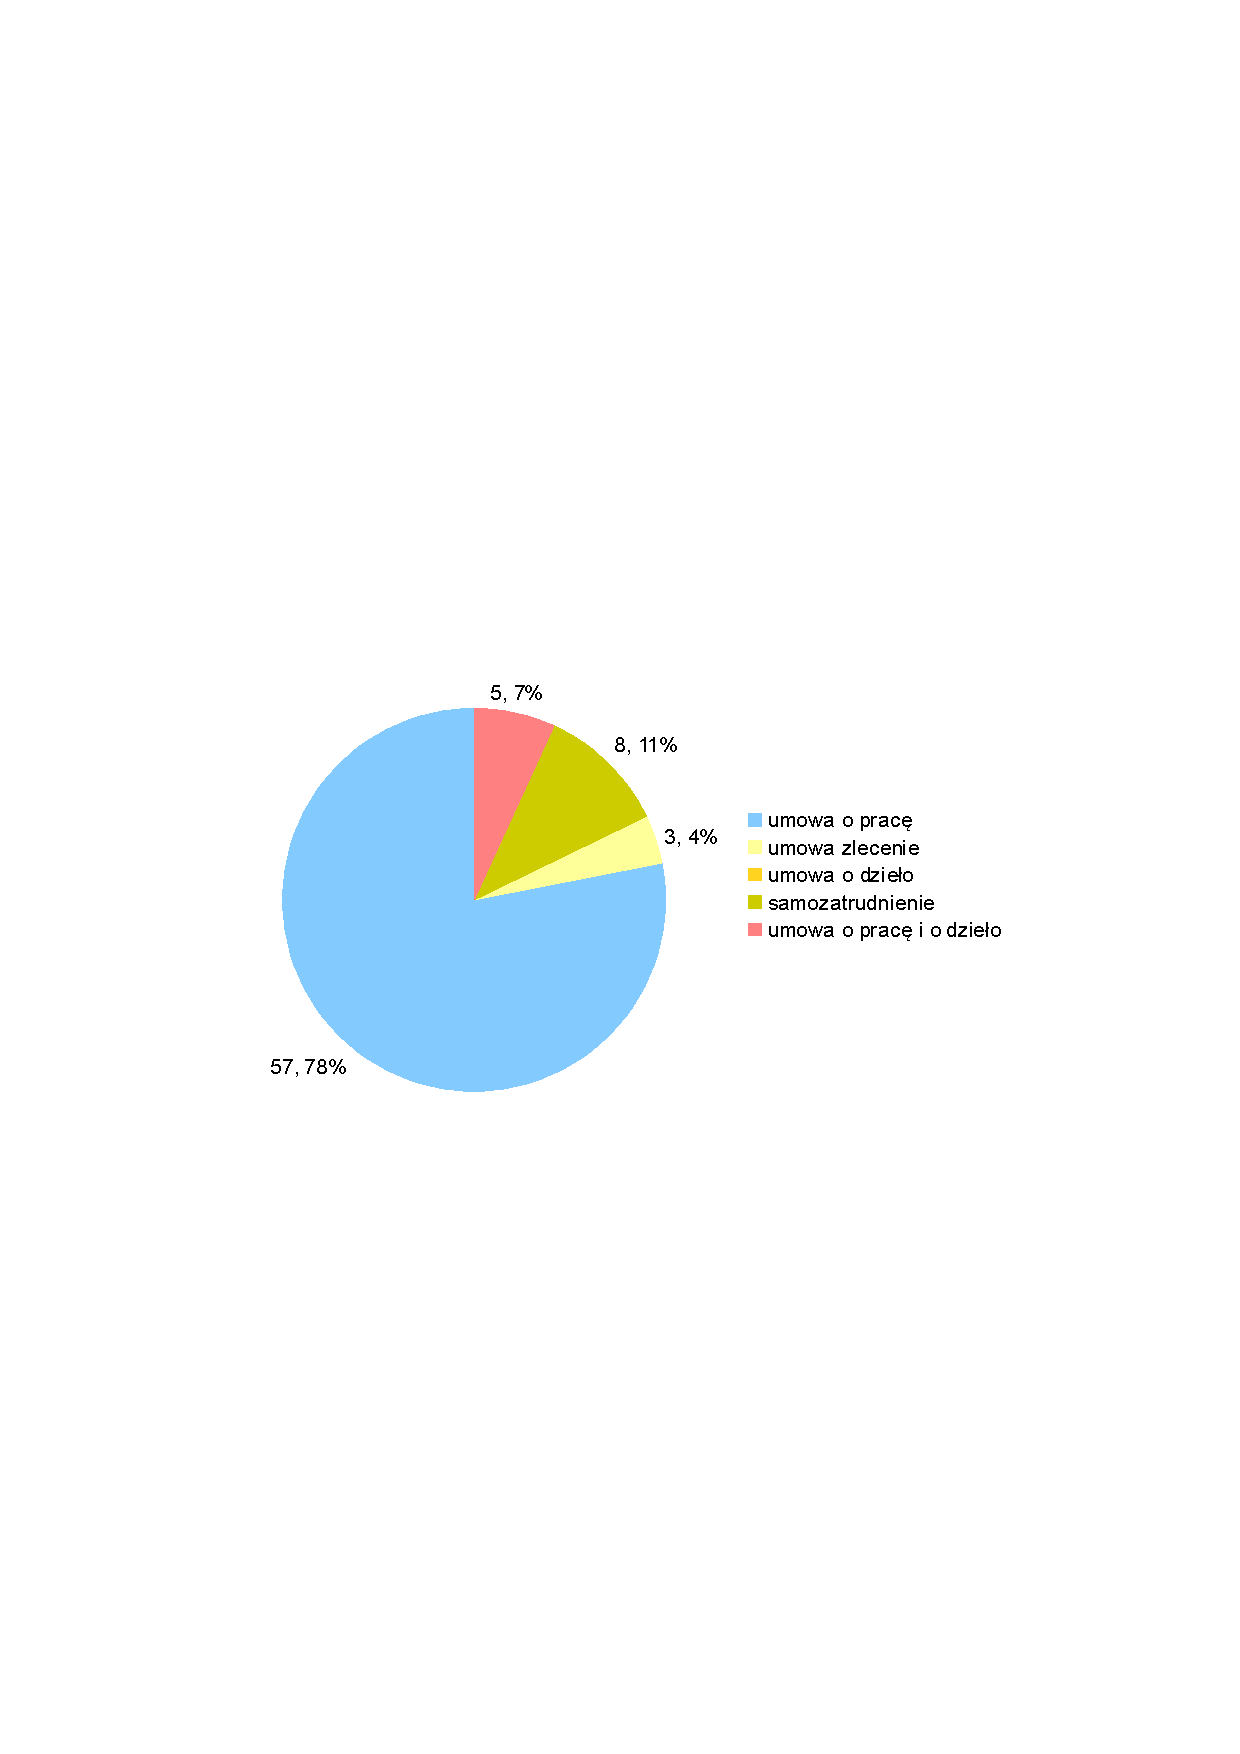
\includegraphics[width=0.8\textwidth]{work-agreement}
\end{center}
\caption{Rodzaj zatrudnienia wśród respondentów.}
\label{fig:work-agreement}
\end{figure}

Z ciekawy wartości jakie pojawiły się w danych, to dla formy umowy, jeżeli respondent wpisywał ,,inne", oznaczało to zawsze jednocześnie umowę o pracę i dzieło (co zostało uwzględnione w Tabeli \ref{tab:work-time-stats}).

\subsection{Charakterystyka firmy}

\begin{table}[h!]
\begin{center}
\begin{tabular}{l l r r}
Typ firmy & Rozmiar & Liczba & Procenty \\ \hline
mikroprzedsiębiorstwo & od 1 do 9 osób & 5 & 6,85\% \\
małe przedsiębiorstwo & od 10 do 49 osób & 11 & 15,07\% \\
średniej wielkości przedsiębiorstwo & od 50 do 249 osób & 15 & 20,55\% \\
duże przedsiębiorstwo & powyżej 250 osób & 42 & 57,53\% \\
\end{tabular}
\end{center}
\caption{Typ i rozmiar firmy respondentów.}
\label{tab:company-size}
\end{table}

\begin{figure}[htb]
\begin{center}
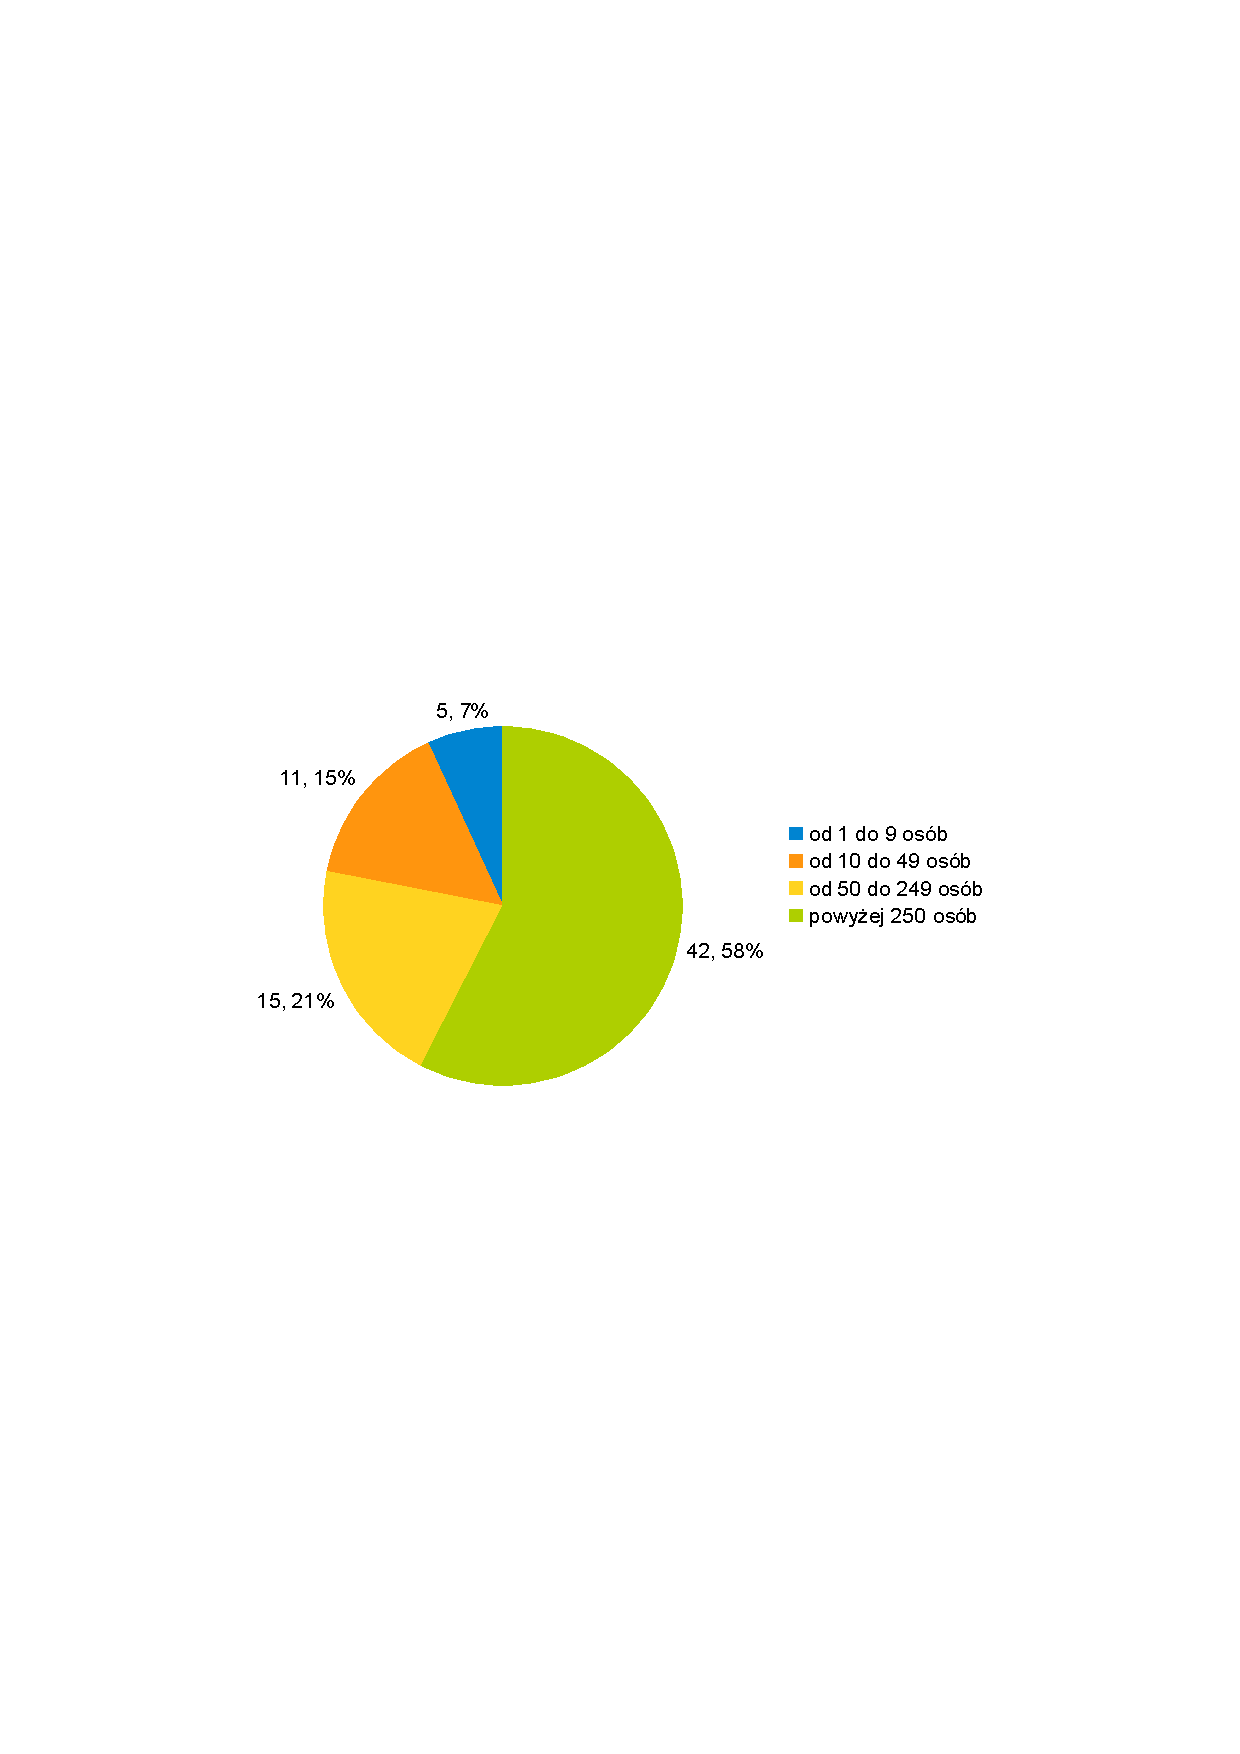
\includegraphics[width=0.8\textwidth]{company-size}
\end{center}
\caption{Rozmiar firmy respondentów.}
\label{fig:company-size}
\end{figure}

Dane z Tabeli \ref{tab:company-size} wskazują, że ponad połowa respondentów pracuje w dużym przedsiębiorstwie. Tylko 5 osób w mikroprzedsiębiorstwie (6,85\%), 11 (15,07\%), a 15 (20,55\%) w średniej wielkości firmie. Czyli w większych organizacjach powyżej 50 pracowników pracuje 78,08\% (57 osób) grupy badanych.

\begin{table}[h!]
\begin{center}
\begin{tabular}{l r r}
Rodzaj firmy & Liczba & Procenty \\ \hline
prywatna firma polska & 17 & 23,29\% \\
firma państwowa & 29 & 39,73\% \\
z udziałem zagranicznym lub polska filia firmy zagranicznej & 20 & 27,40\% \\
organizacja pozarządowa lub non profit & 3 & 4,11\% \\
inne & 4 & 5,48\% \\
\end{tabular}
\end{center}
\caption{Rodzaj firmy respondentów.}
\label{tab:company}
\end{table}

\begin{figure}[htb]
\begin{center}
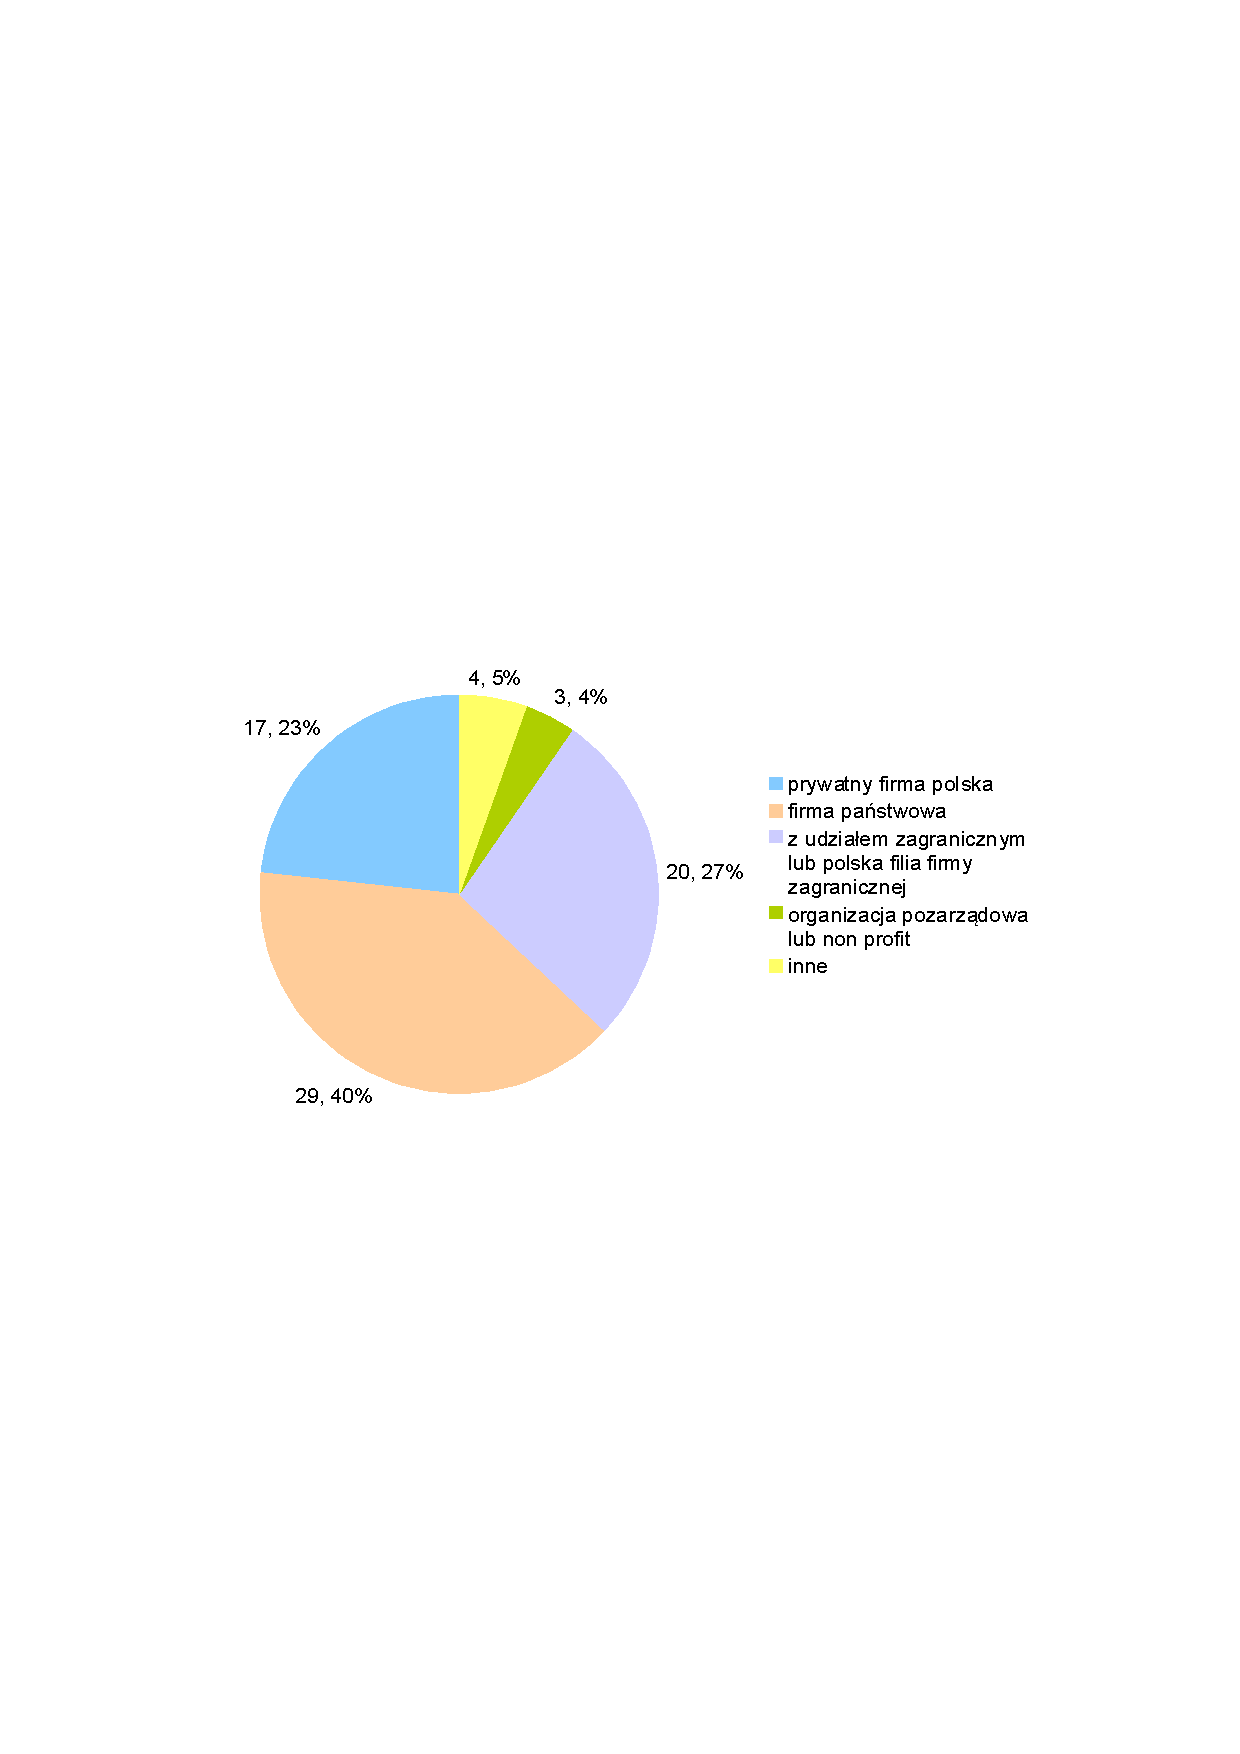
\includegraphics[width=0.8\textwidth]{company}
\end{center}
\caption{Rodzaj firmy respondentów.}
\label{fig:company}
\end{figure}

Patrząc na dane z Tabeli \ref{tab:company} większość respondentów (29 osób; 39,73\%) pracuje dla firmy państwowej. Następne w kolejności są firmy z udziałem zagranicznym -- 20 osób (27,40\%), a tuż za nimi prywatne firmy polskie (23,29\%). Za to tylko 3 osoby (4,11\%) pracuje dla organizacji pozarządowych lub non profit (co nie dziwi ze względu na charakter pracy) oraz 4 osoby (5,48\%) wskazały inne rodzaj firmy.
